\documentclass{standalone}
\usepackage{tikz}
\usetikzlibrary{patterns, positioning}


\begin{document}
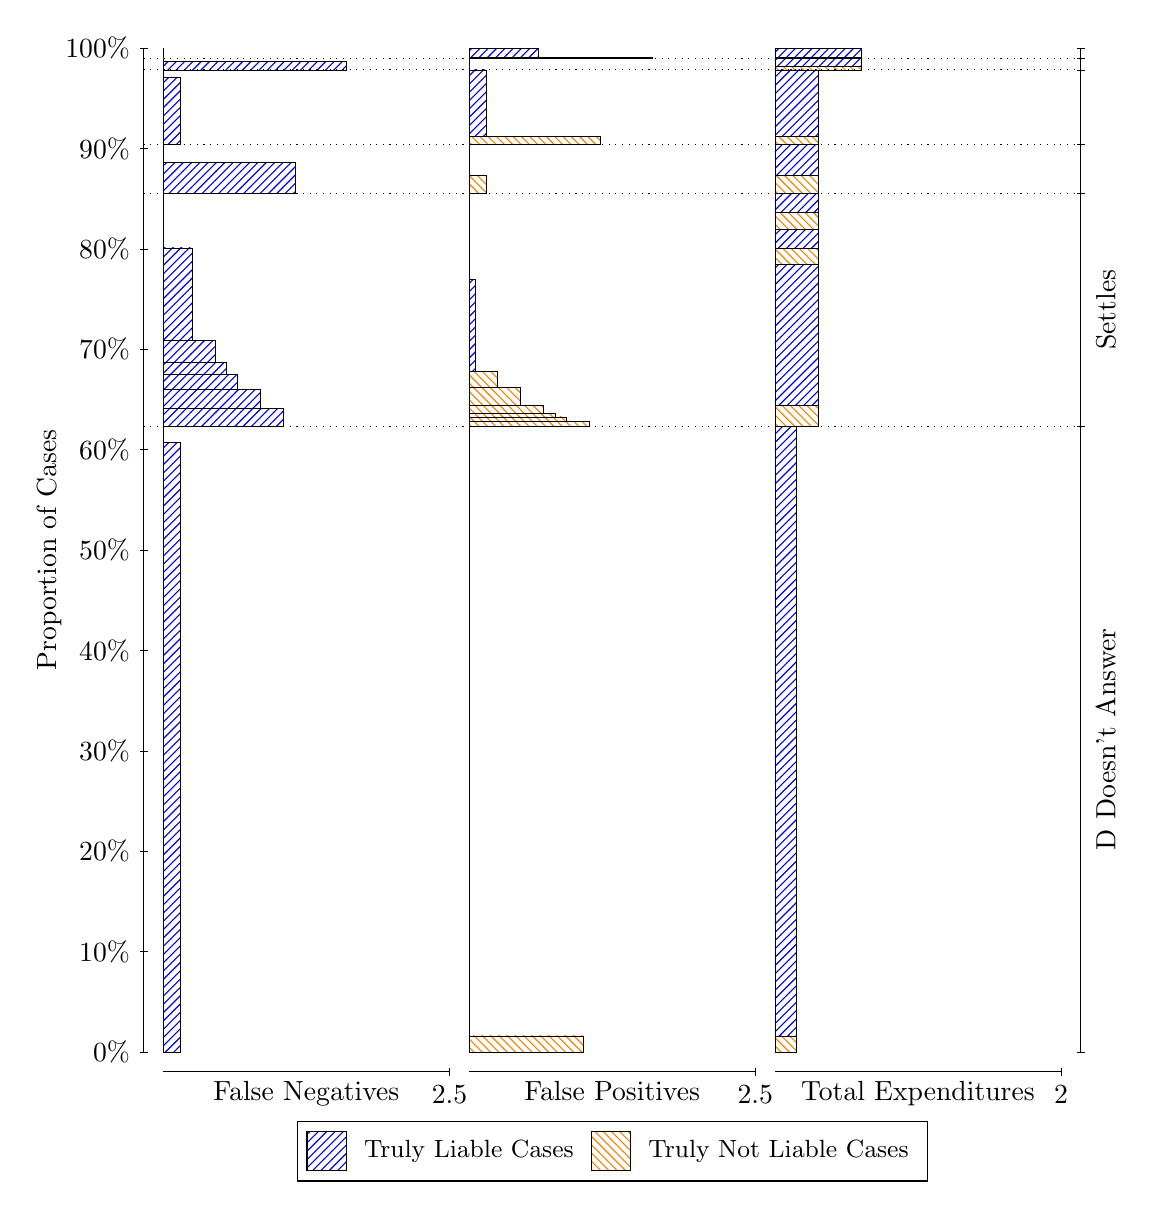
\begin{tikzpicture}
\draw[black, very thin] (1.5,1.75) -- (1.5,14.5);
\node[rotate=90, text=black, anchor=center] at (0.3, 8.125) {Proportion of Cases};
\draw[black, very thin] (1.45,1.75) -- (1.55,1.75);
\node[text=black, anchor=east] at (1.45, 1.75) {0\%};
\draw[black, very thin] (1.45,3.025) -- (1.55,3.025);
\node[text=black, anchor=east] at (1.45, 3.025) {10\%};
\draw[black, very thin] (1.45,4.3) -- (1.55,4.3);
\node[text=black, anchor=east] at (1.45, 4.3) {20\%};
\draw[black, very thin] (1.45,5.575) -- (1.55,5.575);
\node[text=black, anchor=east] at (1.45, 5.575) {30\%};
\draw[black, very thin] (1.45,6.85) -- (1.55,6.85);
\node[text=black, anchor=east] at (1.45, 6.85) {40\%};
\draw[black, very thin] (1.45,8.125) -- (1.55,8.125);
\node[text=black, anchor=east] at (1.45, 8.125) {50\%};
\draw[black, very thin] (1.45,9.4) -- (1.55,9.4);
\node[text=black, anchor=east] at (1.45, 9.4) {60\%};
\draw[black, very thin] (1.45,10.675) -- (1.55,10.675);
\node[text=black, anchor=east] at (1.45, 10.675) {70\%};
\draw[black, very thin] (1.45,11.95) -- (1.55,11.95);
\node[text=black, anchor=east] at (1.45, 11.95) {80\%};
\draw[black, very thin] (1.45,13.225) -- (1.55,13.225);
\node[text=black, anchor=east] at (1.45, 13.225) {90\%};
\draw[black, very thin] (1.45,14.5) -- (1.55,14.5);
\node[text=black, anchor=east] at (1.45, 14.5) {100\%};

\draw[black, very thin] (13.4,1.75) -- (13.4,14.5);
\draw[black, very thin] (13.35,1.75) -- (13.45,1.75);
\node[anchor=west] at (13.35, 1.75) {};
\draw[black, very thin] (13.35,9.6952) -- (13.45,9.6952);
\node[anchor=west] at (13.35, 9.6952) {};
\draw[black, very thin] (13.35,12.657) -- (13.45,12.657);
\node[anchor=west] at (13.35, 12.657) {};
\draw[black, very thin] (13.35,13.277) -- (13.45,13.277);
\node[anchor=west] at (13.35, 13.277) {};
\draw[black, very thin] (13.35,14.222) -- (13.45,14.222);
\node[anchor=west] at (13.35, 14.222) {};
\draw[black, very thin] (13.35,14.369) -- (13.45,14.369);
\node[anchor=west] at (13.35, 14.369) {};
\draw[black, very thin] (13.35,14.5) -- (13.45,14.5);
\node[anchor=west] at (13.35, 14.5) {};

\draw[black, very thin, pattern color=blue, pattern=north east lines] (1.75,1.75) rectangle (1.968,9.492);
\draw[black, very thin, pattern color=orange, pattern=north west lines] (1.75,9.492) rectangle (1.75,9.6952);
\draw[black, very thin, pattern color=blue, pattern=north east lines] (1.75,9.6952) rectangle (3.276,9.9282);
\draw[black, very thin, pattern color=blue, pattern=north east lines] (1.75,9.9282) rectangle (2.9853,10.169);
\draw[black, very thin, pattern color=blue, pattern=north east lines] (1.75,10.169) rectangle (2.6947,10.358);
\draw[black, very thin, pattern color=blue, pattern=north east lines] (1.75,10.358) rectangle (2.5493,10.506);
\draw[black, very thin, pattern color=blue, pattern=north east lines] (1.75,10.506) rectangle (2.404,10.79);
\draw[black, very thin, pattern color=blue, pattern=north east lines] (1.75,10.79) rectangle (2.1133,11.961);
\draw[black, very thin, pattern color=orange, pattern=north west lines] (1.75,11.961) rectangle (1.75,12.657);
\draw[black, very thin, pattern color=blue, pattern=north east lines] (1.75,12.657) rectangle (3.4213,13.052);
\draw[black, very thin, pattern color=orange, pattern=north west lines] (1.75,13.052) rectangle (1.75,13.277);
\draw[black, very thin, pattern color=blue, pattern=north east lines] (1.75,13.277) rectangle (1.968,14.126);
\draw[black, very thin, pattern color=orange, pattern=north west lines] (1.75,14.126) rectangle (1.75,14.222);
\draw[black, very thin, pattern color=blue, pattern=north east lines] (1.75,14.222) rectangle (4.0753,14.327);
\draw[black, very thin, pattern color=orange, pattern=north west lines] (1.75,14.327) rectangle (1.75,14.369);
\draw[black, very thin, pattern color=orange, pattern=north west lines] (1.75,14.369) rectangle (1.75,14.381);
\draw[black, very thin, pattern color=blue, pattern=north east lines] (1.75,14.381) rectangle (1.75,14.5);
\draw[black, very thin, pattern color=orange, pattern=north west lines] (5.6333,1.75) rectangle (7.0867,1.9532);
\draw[black, very thin, pattern color=blue, pattern=north east lines] (5.6333,1.9532) rectangle (5.6333,9.6952);
\draw[black, very thin, pattern color=orange, pattern=north west lines] (5.6333,9.6952) rectangle (7.1593,9.7588);
\draw[black, very thin, pattern color=orange, pattern=north west lines] (5.6333,9.7588) rectangle (6.8687,9.8144);
\draw[black, very thin, pattern color=orange, pattern=north west lines] (5.6333,9.8144) rectangle (6.7233,9.8612);
\draw[black, very thin, pattern color=orange, pattern=north west lines] (5.6333,9.8612) rectangle (6.578,9.9635);
\draw[black, very thin, pattern color=orange, pattern=north west lines] (5.6333,9.9635) rectangle (6.2873,10.189);
\draw[black, very thin, pattern color=orange, pattern=north west lines] (5.6333,10.189) rectangle (5.9967,10.391);
\draw[black, very thin, pattern color=blue, pattern=north east lines] (5.6333,10.391) rectangle (5.706,11.562);
\draw[black, very thin, pattern color=blue, pattern=north east lines] (5.6333,11.562) rectangle (5.6333,12.657);
\draw[black, very thin, pattern color=orange, pattern=north west lines] (5.6333,12.657) rectangle (5.8513,12.882);
\draw[black, very thin, pattern color=blue, pattern=north east lines] (5.6333,12.882) rectangle (5.6333,13.277);
\draw[black, very thin, pattern color=orange, pattern=north west lines] (5.6333,13.277) rectangle (7.3047,13.374);
\draw[black, very thin, pattern color=blue, pattern=north east lines] (5.6333,13.374) rectangle (5.8513,14.222);
\draw[black, very thin, pattern color=orange, pattern=north west lines] (5.6333,14.222) rectangle (5.6333,14.265);
\draw[black, very thin, pattern color=blue, pattern=north east lines] (5.6333,14.265) rectangle (5.6333,14.369);
\draw[black, very thin, pattern color=orange, pattern=north west lines] (5.6333,14.369) rectangle (7.9587,14.381);
\draw[black, very thin, pattern color=blue, pattern=north east lines] (5.6333,14.381) rectangle (6.5053,14.5);
\draw[black, very thin, pattern color=orange, pattern=north west lines] (9.5167,1.75) rectangle (9.7892,1.9532);
\draw[black, very thin, pattern color=blue, pattern=north east lines] (9.5167,1.9532) rectangle (9.7892,9.6952);
\draw[black, very thin, pattern color=orange, pattern=north west lines] (9.5167,9.6952) rectangle (10.062,9.9635);
\draw[black, very thin, pattern color=blue, pattern=north east lines] (9.5167,9.9635) rectangle (10.062,11.756);
\draw[black, very thin, pattern color=orange, pattern=north west lines] (9.5167,11.756) rectangle (10.062,11.958);
\draw[black, very thin, pattern color=blue, pattern=north east lines] (9.5167,11.958) rectangle (10.062,12.192);
\draw[black, very thin, pattern color=orange, pattern=north west lines] (9.5167,12.192) rectangle (10.062,12.417);
\draw[black, very thin, pattern color=blue, pattern=north east lines] (9.5167,12.417) rectangle (10.062,12.657);
\draw[black, very thin, pattern color=orange, pattern=north west lines] (9.5167,12.657) rectangle (10.062,12.882);
\draw[black, very thin, pattern color=blue, pattern=north east lines] (9.5167,12.882) rectangle (10.062,13.277);
\draw[black, very thin, pattern color=orange, pattern=north west lines] (9.5167,13.277) rectangle (10.062,13.374);
\draw[black, very thin, pattern color=blue, pattern=north east lines] (9.5167,13.374) rectangle (10.062,14.222);
\draw[black, very thin, pattern color=orange, pattern=north west lines] (9.5167,14.222) rectangle (10.607,14.265);
\draw[black, very thin, pattern color=blue, pattern=north east lines] (9.5167,14.265) rectangle (10.607,14.369);
\draw[black, very thin, pattern color=orange, pattern=north west lines] (9.5167,14.369) rectangle (10.607,14.381);
\draw[black, very thin, pattern color=blue, pattern=north east lines] (9.5167,14.381) rectangle (10.607,14.5);
\draw[black, dotted] (1.5,9.6952) -- (13.4,9.6952);
\draw[black, dotted] (1.5,12.657) -- (13.4,12.657);
\draw[black, dotted] (1.5,13.277) -- (13.4,13.277);
\draw[black, dotted] (1.5,14.222) -- (13.4,14.222);
\draw[black, dotted] (1.5,14.369) -- (13.4,14.369);
\draw[black, very thin] (1.75,1.5) -- (5.3833,1.5);
\node[text=black, anchor=north] at (3.5667, 1.5) {False Negatives};
\draw[black, very thin] (5.3833,1.45) -- (5.3833,1.55);
\node[text=black, anchor=north] at (5.3833, 1.45) {2.5};

\draw[black, very thin] (5.6333,1.5) -- (9.2667,1.5);
\node[text=black, anchor=north] at (7.45, 1.5) {False Positives};
\draw[black, very thin] (9.2667,1.45) -- (9.2667,1.55);
\node[text=black, anchor=north] at (9.2667, 1.45) {2.5};

\draw[black, very thin] (9.5167,1.5) -- (13.15,1.5);
\node[text=black, anchor=north] at (11.333, 1.5) {Total Expenditures};
\draw[black, very thin] (13.15,1.45) -- (13.15,1.55);
\node[text=black, anchor=north] at (13.15, 1.45) {2};

\node[text=black, centered, rotate=90] at (13.72, 5.7226) {D Doesn't Answer};
\node[text=black, centered, rotate=90] at (13.72, 11.176) {Settles};





\draw (7.449999999999999,1.5) node[draw=none] (baseCoordinate) {};
\begin{scope}[align=center]
        \matrix[scale=0.5, draw=black, below=0.5cm of baseCoordinate, nodes={draw}, column sep=0.1cm]{
            \node[rectangle, draw, minimum width=0.5cm, minimum height=0.5cm, pattern color=blue, pattern=north east lines] {}; &
            \node[draw=none, font=\small, text=black] (B) {Truly Liable Cases}; &
            \node[rectangle, draw, minimum width=0.5cm, minimum height=0.5cm, pattern color=orange, pattern=north west lines] {}; &
            \node[draw=none, font=\small, text=black] (B) {Truly Not Liable Cases}; \\
            };
\end{scope}

\end{tikzpicture}
\end{document}